\documentclass[11pt,a4paper]{article}
\usepackage[utf8]{inputenc}
\usepackage[french]{babel}
\usepackage{amsmath}
\usepackage{amsthm}
\usepackage{amsfonts}
\usepackage{xcolor}
\usepackage{amssymb}
\usepackage{graphicx}
\usepackage{hyperref}
\usepackage{lscape} % pdflscape

\hypersetup{
    colorlinks=true,
    linkcolor=red,
    filecolor=magenta,      
    urlcolor=red,
    pdftitle={Rapport - PAP - Black & Scholes},
    pdfpagemode=FullScreen,
    }
\usepackage{stmaryrd}
\usepackage{minted}


\usepackage{relsize}
\usepackage{listings}
\usepackage{courier}
\usepackage[left=3.2cm,right=3.2cm,top=3.2cm,bottom=3.2cm]{geometry}
\usepackage{fancyhdr}

%\pagestyle{fancy}
%\title{Rapport final - Projet PAP\\Programmation avancée \& }
\title{\textbf{Rapport - Programmation Avancée \& Projet} \\[0.2em]\smaller{} Etude et Implémentation de l'équation de Black et Scholes}

\author{\textbf{Lucas RODRIGUEZ}}
\date{Janvier 2022}

\newcommand{\deriv}[3][]{% \deriv[<order>]{<func>}{<var>}
  \ensuremath{\frac{\partial^{#1} {#2}}{\partial {#3}^{#1}}}}
\newcommand*{\intval}[2]{\llbracket #1, #2 \rrbracket}
\newcommand*{\C}[2]{\mathbf{C}^{#1}_{#2}}

\theoremstyle{plain}
\newtheorem{rmq}{Remarque}
\newtheorem{prop}{Proposition}
\DeclareMathOperator{\R}{\mathbb{R}}

\renewcommand\qedsymbol{$\blacksquare$}

\begin{document}

\maketitle

\section*{Introduction}
Ce rapport a pour but de présenter notre travail sur le projet de l'UE Programmation Avancée \& Projet.
Nous avons choisi de réaliser ce projet sur le sujet n°2 concernant la \textbf{simulation de l'équation de Black et Scholes}. Le présent document présente nos pistes de travail, les difficultés techniques et mathématiques rencontrées, les solutions proposées puis implémentées pour aboutir à un programme informatique répondant aux attentes du sujet.

\paragraph{Objectif du sujet \& Plan} Dans un premier temps, nous réalisons un important travail bibliographique autour de l'équation de Black-Scholes, puis des méthodes des différences finies. Notre attention s'est plus particulièrement portée sur les discrétisations implicite et de Crank-Nicholson.
Après avoir appliqué ces méthodes sur les EDP présentées, un travail sur la structure technique est réalisé au travers de la conception d'un diagramme de classes. Cette étape permet ainsi de prévoir au mieux les différentes imbrications de notre implémentation de la solution en C++.


\tableofcontents



\newpage 


\section{Prospection \& travaux théoriques}

\subsection{Equation de Black-Scholes}
On note la fonction $C : \left[0, T\right]\times\left[0, L\right] \longrightarrow \R$. Il s'agit de la solution de l'EDP complète de Black-Scholes 

L'équation de Black Scholes est intialement présentée sous la forme suivante :
\begin{equation}
    \label{eq:EDP_complete}
    \deriv{C}{t} + rS\deriv{C}{S} + \frac{1}{2}\sigma^2S^2\deriv[2]{C}{S} - rC = 0, \ \forall (t, S) \in \left[0, T\right]\times\left[0, L\right]
\end{equation}
Elle est qualifiée de \textbf{complète}.

Après changement de variable sur $C$, nous pouvons \og approximer \fg \ l'EDP complète par une EDP dite \textbf{réduite} :

\begin{equation}
\label{eq:EDP_reduite}
    \deriv{\widetilde{C}}{\widetilde{t}} = \mu \deriv[2]{\widetilde{C}}{\widetilde{S}}, \ \forall (\widetilde{t}, \widetilde{S}) \in \left[0, T\right]\times\left[0, L\right]
\end{equation}

La solution de l'EDP réduite est alors $\widetilde{C}$, approximation de $C$ et $\mu \in \R$.


\begin{rmq}[Valeur de $\mu$] La première remarque que l'on peut se faire est relative à la valeur numérique de $\mu$. Comme cette dernière n'est pas donnée dans le sujet, il va falloir la déterminer.
\end{rmq}

\begin{rmq}[Analogie avec la thermodynamique]
Nous pouvons égalemement noter que l'EDP réduite \eqref{eq:EDP_reduite} est semblable à l'équation de la chaleur, le nombre $\mu$ étant le \underline{coefficient de diffusivité thermique}.
\end{rmq}


\subsection{Détermination du coefficient $\mu$}

\begin{prop}[Valeur du coefficient $\mu$] $$\boxed{\mu = \frac{1}{2}\sigma^2} \in \R$$
\end{prop}

Comme indiqué dans l'énoncé, la transformation de \eqref{eq:EDP_complete} à \eqref{eq:EDP_reduite} implique un, voire plusieurs changements de variables.


On peut montrer que l'équation \eqref{eq:EDP_complete} est équivalente à une autre expression nous permettant plus facilement de déterminer $\mu$.

\begin{align}
    \deriv{C}{t} + \frac{1}{2}\sigma^2 S^2 \deriv[2]{C}{S} + rS\deriv{C}{S} - rC &= 0 \tag{1} \\
    \Longleftrightarrow \deriv{C}{t} + \frac{1}{2}\sigma^2\Big(S\deriv{}{S}\Big)^2C + \Big(r - \frac{1}{2}\sigma^2\Big)S\deriv{C}{S} - rC &= 0 \label{3}
\end{align}

\begin{proof}
En effet, en utilisant la règle du produit de différentielles sur l'opérateur $S\deriv{}{S}$, on obtient :

$$
\Big(S\deriv{}{S}\Big)^2C = S\deriv{}{S}\Big(S\deriv{C}{S}\Big) = S\Big(\deriv{S}{S}\deriv{C}{S} + S\deriv[2]{C}{S}\Big) = S\deriv{C}{S} + S^2\deriv[2]{C}{C}
$$
En injectant ce résultat dans \eqref{3}, on a :

\begin{align*}
    \deriv{C}{t} + \frac{1}{2}\sigma^2\Big(S\deriv{C}{S} + S^2\deriv[2]{C}{S}\Big) + \Big(r - \frac{1}{2}\sigma^2\Big)S\deriv{C}{S} - rC &= 0 \\
    \Longleftrightarrow \deriv{C}{t} + \frac{1}{2}\sigma^2S^2\deriv[2]{C}{S} + rS\deriv{C}{S} - rC &= 0
\end{align*}
On retrouve l'équation \eqref{eq:EDP_complete}. 


On effectue un premier changement de variables : $\psi : (t, S) \longrightarrow (\tau, y)$ avec : $S = \exp y$ et $t = T - \tau$.

L'application $\psi$ est de classe $\mathcal{C}^1$ donc différentiable sur $\R^2$.

Ainsi : 
$$
\boxed{S\deriv{\bullet}{S} \longrightarrow \deriv{\bullet}{y}} \ \text{et} \ \boxed{\deriv{\bullet}{t} \longrightarrow -\deriv{\bullet}{\tau}}
$$

En appliquant $\psi$ à \eqref{3}, on a :



\begin{align*}
    -\deriv{C}{\tau} + \frac{1}{2}\sigma^2\deriv[2]{C}{y} + \Big(r - \frac{1}{2}\sigma^2\Big)\deriv{C}{y} - rC &= 0 \\
    \Longleftrightarrow \deriv{C}{\tau} - \frac{1}{2}\sigma^2\deriv[2]{C}{y} - \Big(r - \frac{1}{2}\sigma^2\Big)\deriv{C}{y} + rC &= 0
\end{align*}

Si on fixe $u = \exp(r\tau)C$, alors dans \eqref{3} :
$$
u = \exp(r\tau)C \Longrightarrow \boxed{C = u\exp(-r\tau) \Longrightarrow \deriv{C}{\tau} = -r\Big(\deriv{u}{\tau}\Big)\exp(-r\tau)}
$$

On obtient :
\begin{align*}
    -\Big(\deriv{u}{\tau}e^{-r\tau} + (-r)e^{-r\tau}u\Big) + \frac{1}{2}\sigma^2 e^{-r\tau}\deriv[2]{u}{y} + \Big(r - \frac{1}{2}\sigma^2\Big)e^{-r\tau}\deriv{u}{y} - rue^{-r\tau} &= 0 \\
    -\deriv{u}{\tau}e^{-r\tau} + \frac{1}{2}\sigma^2e^{-r\tau}\deriv[2]{u}{y} + \Big(r - \frac{1}{2}\sigma^2\Big)\deriv{u}{y}e^{-r\tau} &= 0 \\
    \deriv{u}{\tau} - \frac{1}{2}\sigma^2\deriv[2]{u}{y} - \Big(r - \frac{1}{2}\sigma^2\Big)\deriv{u}{y} &= 0
\end{align*}

On réalise un autre changement de variable :
$$
\boxed{\widetilde{S} = y + \Big(r - \frac{1}{2}\sigma^2\Big)\widetilde{t}} \ \text{et} \ \boxed{\widetilde{t} = \tau}
$$

On a :

$$
\deriv{\bullet}{\widetilde{S}} = \deriv{\bullet}{\tau}\deriv{\tau}{\widetilde{S}} + \deriv{\bullet}{y}\deriv{y}{\widetilde{S}} = \deriv{\bullet}{y}
$$

et 
$$
\deriv{\bullet}{\widetilde{t}} = \deriv{\bullet}{\tau}\deriv{\tau}{\widetilde{t}} + \deriv{\bullet}{y}\deriv{y}{\widetilde{t}} = \deriv{\bullet}{\tau} + \deriv{\bullet}{y}(-1)\Big(r - \frac{1}{2}\sigma^2\Big) = \deriv{\bullet}{\tau} - \deriv{\bullet}{y}\Big(r - \frac{1}{2}\sigma^2\Big)
$$
car $y = \widetilde{S} - (r - \frac{1}{2}\sigma^2)\widetilde{t}$

d'où :

$$
\deriv{u}{\widetilde{t}} + (r - \frac{1}{2}\sigma^2)\deriv{u}{y} - \frac{1}{2}\sigma^2\deriv[2]{u}{\widetilde{S}} - \Big(r - \frac{1}{2}\sigma^2\Big)\deriv{u}{y} = 0
$$

d'où en simplifiant :

$$
\Longrightarrow \deriv{u}{\widetilde{t}} = \frac{1}{2}\sigma^2\deriv[2]{u}{\widetilde{S}}
$$
D'où le résultat en identifiant $u$ à $\widetilde{C}$. Par identification, on obtient $\boxed{\mu = \frac{1}{2}\sigma^2}$.
\end{proof}




\subsection{Présentation du domaine de résolution}
On pose $\mathcal{D} = \left[0, T\right]\times\left[0, L\right]$.

Nous effectuons une discrétisation du domaine $\mathcal{D}$.

\begin{itemize}
    \item $\forall m \in \intval{0}{M}, \boxed{t_m = m\Delta t}$ avec : $\Delta t = \frac{T}{M}$
    \item $\forall j \in \intval{0}{N}, \boxed{s_j = j\Delta s}$ avec : $\Delta s = \frac{L}{N}$
\end{itemize}

\begin{figure}[h]
    \centering
    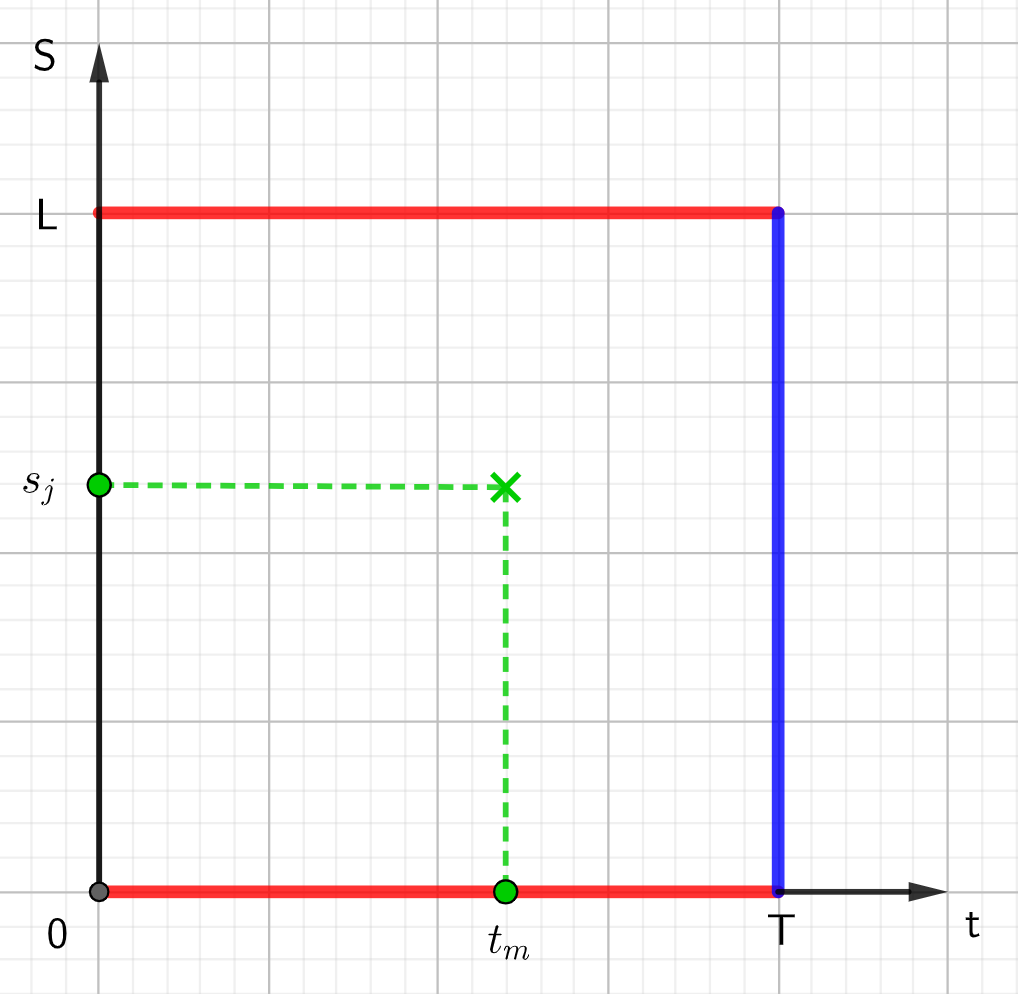
\includegraphics[scale=0.23]{img/situation_diagram.png}
    \caption{Domaine de résolution sur $\mathcal{D}$}
    \label{fig:domaine}
\end{figure}

Sur \ref{fig:domaine}, on peut noter :
\begin{itemize}
    \item Les \textcolor{red}{\textbf{segments rouges}} représentent les conditions aux bords.
    \begin{itemize}
        \item Celle en $S = 0$ est appelée condition aux bords basse
        \item Celle en $S = L$ est appelée condition aux bords haute
    \end{itemize}
    \item Le \textcolor{blue}{\textbf{segment bleu}} représente la condition terminale.
\end{itemize}

L'objectif est de déterminer puis de tracer graphiquement les nuages de points $$\lbrace (s_j, C(0, s_j)), \forall j \in \intval{0}{N} \rbrace \ \text{et} \ \lbrace (s_j, \widetilde{C}(0, s_j)), \forall j \in \intval{0}{N} \rbrace$$



Par la suite, on notera $\mathbf{C}^{m}_j$, la quantité $C(t_m, s_j)$.


\subsection{Etude de l'EDP complète (schéma de Crank-Nicholson)}
Le schéma de Crank-Nicholson est un $\theta$-schéma avec $\theta = \frac{1}{2}$. Il s'agit de la moyenne arithmétique entre la méthode explicite et la méthode implicite (décrite dans la section suivante).

Nous commençons par discrétiser les différentes composantes intervenants au sein de l'équation \eqref{eq:EDP_complete} :
\begin{align*}
    C(t, s) &\simeq \C{m}{j} \\
    \deriv{C}{t} &\simeq \frac{1}{\Delta t}\Big(\C{m + 1}{j} - \C{m}{j}\Big) \\
    \deriv{C}{S} &\simeq \frac{1}{4\Delta s}\Big(\C{m + 1}{j + 1} - \C{m + 1}{j - 1} + \C{m}{j + 1} - \C{m}{j - 1}\Big) \\
    \deriv[2]{C}{S} &\simeq \frac{1}{2(\Delta s)^2}\Big(\C{m + 1}{j + 1} - 2\C{m + 1}{j} + \C{m + 1}{j - 1} + \C{m}{j + 1} - 2\C{m}{j} + \C{m}{j - 1}\Big)
\end{align*}
Nous pouvons ensuite injecter ces discrétisations au sein de \eqref{eq:EDP_complete} : $\forall (m, j) \in \intval{0}{M - 1} \times \intval{1}{N - 1}$, 

\begin{align*}
    \frac{1}{\Delta t}\Big(\C{m + 1}{j} - \C{m}{j}\Big) + \frac{rj}{4}\Big(\C{m + 1}{j + 1} - \C{m + 1}{j - 1} + \C{m}{j + 1} - \C{m}{j - 1}\Big) + \\
\frac{1}{4}\sigma^2j^2\Big(\C{m + 1}{j + 1} - 2\C{m + 1}{j} + \C{m + 1}{j - 1} + \C{m}{j + 1} - 2\C{m}{j} + \C{m}{j - 1}\Big) - r\C{m}{j} = 0
\end{align*}
On sépare les termes de temps $t_{m + 1}$ et $t_m$ :

\begin{align*}
    \frac{1}{\Delta t}\C{m + 1}{j} + \frac{rj}{4}\Big(\C{m + 1}{j + 1} - \C{m + 1}{j - 1}\Big) + \frac{\sigma^2j^2}{4}\Big(\C{m + 1}{j + 1} - 2\C{m + 1}{j} + \C{m + 1}{j - 1}\Big) = \\
    \frac{1}{\Delta t}\C{m}{j} - \frac{rj}{4}\Big(\C{m}{j + 1} - \C{m}{j - 1}\Big) - \frac{\sigma^2j^2}{4}\Big(\C{m}{j + 1} - 2\C{m}{j} + \C{m}{j - 1}\Big) + r\C{m}{j}
\end{align*}
On multiplie par $\Delta t$ pour simplifier puis on regroupe les différents termes :

\begin{align*}
    \C{m + 1}{j}\Big[1 - \frac{\sigma^2j^2\Delta t}{2} \Big] + \C{m + 1}{j + 1}\Big[\frac{rj\Delta t}{4} + \frac{\sigma^2j^2\Delta t}{4}\Big] + \C{m + 1}{j - 1}\Big[-\frac{rj\Delta t}{4} + \frac{\sigma^2j^2\Delta t}{4}\Big] = \\
    \C{m}{j}\Big[1 + \frac{\sigma^2j^2\Delta t}{2} + r\Delta t\Big] + \C{m}{j + 1}\Big[-\frac{rj\Delta t}{4} - \frac{\sigma^2j^2\Delta t}{4}\Big] + \C{m}{j - 1}\Big[\frac{rj\Delta t}{4} - \frac{\sigma^2j^2\Delta t}{4}\Big]
\end{align*}
On met en place des coefficients pour faciliter l'écriture de l'expression :

\begin{equation*}
    a_j\C{m + 1}{j - 1} + b_j\C{m + 1}{j} + c_j\C{m + 1}{j + 1} = e_j\C{m}{j - 1} + d_j\C{m}{j} + f_j\C{m}{j + 1} 
\end{equation*}
avec : $\forall j \in \intval{1}{N - 1}$ : 
\begin{align*}
    a_j &= \frac{j\Delta t}{4}\Big(\sigma^2j - r\Big) \\
    b_j &= 1 - \frac{1}{2}\sigma^2j^2\Delta t \\
    c_j &= \frac{j\Delta t}{4}\Big(\sigma^2j + r\Big) \\
    d_j &= 1 + \frac{1}{2}\sigma^2j^2\Delta t + r\Delta t \\
    e_j &= -a_j \\
    f_j &= -c_j
\end{align*}

Afin de résoudre cette équation, on résoud le système matriciel suivant\footnote{Une transformation matricielle préliminaire a été réalisée afin de se trouver avec des matrices carrées propices à la résolution d'un système linéaire} :

$$
\underbrace{\begin{pmatrix}
b_1 & c_1 & 0 & \dots & 0  \\
a_2 & b_2 & \ddots  & \ddots & \vdots  \\
0 & \ddots &\ddots  &\ddots  & 0  \\
\vdots & \ddots & \ddots &\ddots  & c_{N - 2} \\
0 & \dots  & 0  & a_{N - 1} & b_{N - 1} 
\end{pmatrix}}_{\in \mathcal{M}_{N - 1}(\R)}
\underbrace{\begin{pmatrix}
\C{m + 1}{1} \\
\vdots \\
\vdots \\
\vdots \\
\C{m + 1}{N - 1}
\end{pmatrix}}_{\in \R^{N - 1}}
+ 
\underbrace{\begin{pmatrix}
a_{1}(\C{m + 1}{0} + \C{m}{0})\\
0 \\
\vdots \\
0 \\
c_{N - 1}(\C{m + 1}{N} + \C{m}{N})
\end{pmatrix}}_{\in \R^{N - 1}}
=
$$

$$
\underbrace{\begin{pmatrix}
d_1 & -c_1 & 0 & \dots & 0  \\
-a_2 & d_2 & \ddots  & \ddots & \vdots  \\
0 & \ddots &\ddots  &\ddots  & 0  \\
\vdots & \ddots & \ddots &\ddots  & -c_{N - 2} \\
0 & \dots  & 0  & -a_{N - 1} & d_{N - 1} 
\end{pmatrix}}_{\in \mathcal{M}_{N - 1}(\R)}
\underbrace{\begin{pmatrix}
\C{m}{1} \\
\vdots \\
\vdots \\
\vdots \\
\C{m}{N - 1}
\end{pmatrix}}_{\in \R^{N - 1}}
$$
On tombe sur le système matriciel :
$$\boxed{M_1\C{m + 1}{} + k_{m + 1} = M_2\C{m}{}}$$

\begin{rmq}[Observation sur la structure des matricies $M_1$ et $M_2$]
On constate que les matrices $M_1$ et $M_2$ sont des matrices creuses. Par conséquent, leur stockage en mémoire requiert initialement $(N - 1)^2$. Comme $N \sim 10^3$, il est \textbf{non pertinent} de stocker $10^6$ coefficients.

\textbf{\underline{Solution}} : Par conséquent, il est cohérent de ne stocker que les bandes diagonales de coefficients :
\begin{align*}
    A &= (a_1, \ldots, a_{N - 1}) \in \R^{N - 1} \\
    B &= (b_1, \ldots, b_{N - 1}) \in \R^{N - 1} \\
    C &= (c_1, \ldots, c_{N - 1}) \in \R^{N - 1} \\
    D &= (d_1, \ldots, d_{N - 1}) \in \R^{N - 1}
\end{align*}
\end{rmq}

\begin{rmq}[Calcul de $a_j, b_j, c_j, d_j$]
Ces coefficients dépendent de la valeur de $j$ et en C++, les indices vont de $0$ à $N -2$ tandis que nous avons besoin des indices de $1$ à $N - 1$. Il faut donc penser à translater la situation lors du calcul des coefficients des matrices $M_1$ et $M_2$. 
\end{rmq}
La condition terminale s'applique une seule et unique fois\footnote{lors de l'initialisation de l'algorithme.} sur le vecteur $\C{m}{}$.

Les conditions aux bords exigent le calcul du vecteur $k_{m + 1}, \forall m \in \intval{0}{M}$. Ce calcul est donc dépendant du temps; il faut donc actualiser le vecteur à chaque itération.

\begin{rmq}$M_1$ et $M_2$ sont tridiagonales \textbf{et} inversibles.
\end{rmq}

\paragraph{Protocole de résolution numérique} Afin de résoudre les systèmes linéaires $\forall m \in \intval{0}{M}$, plusieurs méthodes de résolution peuvent être adoptées :

Problème : Résoudre $${M_1\C{m + 1}{} + k_{m + 1} = M_2\C{m}{}}, \forall m \in \intval{0}{M}$$
où $\C{m}{}$ est le vecteur d'inconnues.

\begin{itemize}
    \item \textbf{\textcolor{blue}{\underline{Solution 1}} - Simple inversion de matrice} :
On peut implémenter tout d'abord la méthode du pivot de Gauss afin d'inverser tout simplement la matrice $M_2 \in \mathcal{M}_{N - 1}$.

Ainsi :
$$\forall m \in \intval{0}{M}, \ \C{m}{} = M_2^{-1}\Big(M_1\C{m + 1}{} + k_{m + 1}\Big)$$

Néanmoins, pour chaque étape, le coût de cette méthode est en $\mathcal{O}(N^3)$
($\frac{2}{3}N^3 + \textcolor{red}{\textbf{toi}}$\footnote{\textcolor{red}{\textbf{toi}} : termes d'ordre inférieur} opérations). Nous avons cherché à affiner le coût de la méthode.

\item \textbf{\textcolor{blue}{\underline{Solution 2}} - Décomposition LU pour matrice tridiagonale} :
Afin de limiter le coût des opérations, on peut réaliser une décomposition LU de $M_2$ \textbf{une seule fois} lors de l'initialisation.

$$M_2 = LU$$
avec $L$ matrice triangulaire inférieure à diagonale unitaire et $U$ matrice triangulaire supérieure.

Pour ainsi résoudre $M_2x = b$ et qu'on a $M_2 = LU$, on résoud $Ly = b$ puis $Ux = y$.

Pour chaque étape, le coût de cette méthode est en $\mathcal{O}(N^2)$ ($2N^2 + \textcolor{red}{\textbf{toi}}$ opérations).

\vspace{3mm}

\begin{rmq}[Solutions algorithmiques]
On peut utiliser l'algorithme de Doolittle ou de Crout afin de calculer la décomposition LU souhaitée.
\end{rmq}

\item \textbf{\textcolor{blue}{\underline{Solution 3}} - Algorithme de Thomas (résolution de système tridiagonal} :
L'algorithme de Thomas permet de résoudre les systèmes de la forme $Ax = b$ avec $A$ est tridiagonale.

\vspace{3mm}

\begin{rmq}[Avantage au niveau du stockage]
Cette méthode ne requiert pas d'avoir rempli un objet de type \mintinline{cpp}{double**} mais simplement le remplissage des bandes $A, B, C$ et $D$.
\end{rmq}

\vspace{2mm}

Cette méthode possède un côut linéaire : $\mathcal{O}(N)$.
\end{itemize}

Après plusieurs tentatives d'implémentations, nous avons finalement décidé de mettre en place l'algorithme de Thomas pour des considérations d'optimisation du programme final.

\subsection{Etude de l'EDP réduite (schéma implicite)}

Au point $(t_m, s_j)$, on discrétise les différentes composantes différentielles par :

\begin{align*} 
\deriv{\widetilde{C}}{\widetilde{t}} &\simeq \frac{1}{\Delta t}\Big(\C{m + 1}{j} - \C{m}{j}\Big) \\ 
\deriv[2]{\widetilde{C}}{\widetilde{S}} &\simeq \frac{1}{(\Delta s)^2}\Big(\C{m + 1}{j + 1} - 2\C{m + 1}{j} + \C{m + 1}{j - 1}\Big)
\end{align*}

On peut alors injecter les discrétisations de ces deux composantes différentielles dans \eqref{eq:EDP_reduite} :

\begin{align*}
    \frac{1}{\Delta t}\Big(\C{m + 1}{j} - \C{m}{j}\Big) - \frac{\mu}{(\Delta s)^2}\Big(\C{m + 1}{j + 1} - 2\C{m + 1}{j} + \C{m + 1}{j - 1}\Big) &= 0 \\
    \frac{1}{\Delta t}\C{m + 1}{j} - \frac{\mu}{(\Delta s)^2}\Big(\C{m + 1}{j + 1} - 2\C{m + 1}{j} + \C{m + 1}{j - 1}\Big) &= \frac{1}{\Delta t}\C{m}{j} \\
    \C{m + 1}{j}\Big(1 + 2\frac{\mu\Delta t}{(\Delta s)^2}\Big) + \C{m + 1}{j + 1}\Big(-\frac{\mu\Delta t}{(\Delta s)^2}\Big) + \C{m + 1}{j - 1}\Big(-\frac{\mu\Delta t}{(\Delta s)^2}\Big)  &= \C{m}{j}
\end{align*}

Au final, on trouve $\forall (m, j) \in \intval{0}{M} \times \intval{0}{N}$ :
$$\boxed{\C{m}{j} = \C{m + 1}{j}\Big(1 + 2\frac{\mu\Delta t}{(\Delta s)^2}\Big) + \C{m + 1}{j + 1}\Big(-\frac{\mu\Delta t}{(\Delta s)^2}\Big) + \C{m + 1}{j - 1}\Big(-\frac{\mu\Delta t}{(\Delta s)^2}\Big)}
$$
Pour plus de clarté, on peut noter $\alpha = \frac{\mu\Delta t}{(\Delta s)^2}$ d'où :
$$\boxed{\C{m}{j} = - \alpha\C{m + 1}{j - 1} + \Big(1 + 2\alpha\Big)\C{m + 1}{j} - \alpha \C{m + 1}{j + 1}}
$$
En notation matricielle, on obtient :
$$
M_1 = 
\begin{pmatrix}
b & c & 0 & \dots & 0  \\
a & \ddots & \ddots  & \ddots & \vdots  \\
0 & \ddots &\ddots  &\ddots  & 0  \\
\vdots & \ddots & \ddots &\ddots  & c \\
0 & \dots  & 0  & a & b 
\end{pmatrix} \in \mathcal{M}_{N - 1}(\R)
$$
avec $a = c = -\alpha$ et $b = 1 + 2\alpha$. De plus, on note :
$$
\C{m}{} = (\C{m}{1}, \dots, \C{m}{N - 1})^{\textbf{T}} \in \R^{N - 1} \ \text{et} \
k_{m} = (a_1\C{m}{0}, 0, \dots, 0, c_{N - 1}\C{m}{N})^{\textbf{T}} \in \R^{N - 1}
$$


On possède le système suivant :
$$\boxed{M_1\C{m+1}{} + k_{m + 1}= \C{m}{}}$$
\paragraph{Protocole de résolution numérique} Comme détaillé précédemment dans le cadre de l'EDP complète, nous allons utiliser l'algorithme de Thomas afin de résoudre les $M$ systèmes matriciels linéaires.

Cela nous permet d'obtenir un \textbf{coût opérationel linéaire} pour chacune des étapes de l'algorithme; ce qui est très avantageux comparé au côut cubique d'une implémentation du pivot de Gauss.

\section{Implémentation de la solution}
La composition structurelle détaillée du projet est visible à la fois sur le diagramme de classes UML disponible à la fin du rapport ou dans le répertoire \verb|docs/img/| du projet.
\\
De plus, le projet a été entièrement commenté en utilisant la syntaxe de Doxygen. Cette dernière est trouvable au format HTML et \TeX \ dans le répertoire \verb|documentation/|.

\subsection{Gestion des structures de données}
Afin de gérer au mieux les différentes structures de données utilisées au sein de l'implémentation, nous avons créer plusieurs classes et structures en C++ afin de regrouper les informations entre elles.

Nous avons implémenté les classes  suivantes afin
\begin{itemize}
    \item \textbf{\textcolor{blue}{Matrix}} Il s'agit d'un alias du type \mintinline{cpp}{double**}. En effet, nous avons jugé pertinent de ne pas implémenter une véritable classe \mintinline{cpp}{class Matrix} car nous avons estimé que les opérations à réaliser sur le tableau de données étaient élémentaires et que nous garantissions dès le début qu'aucune exception n'allait être levée (ex : indice incorrect, ...).
    \\ Par conséquent, nous avons symplement : \mintinline{cpp}{typedef double** Matrix;}
    \item \textbf{\textcolor{blue}{Mesh}} : Cette classe permet de gérer la création et l'accès aux éléments d'une discrétisation temporelle ou spatiale (selon les besoins de l'opérateur).
    \item \textbf{\textcolor{blue}{Payoff}} : Il s'agit d'une classe abstraite permettant d'implémenter le type de payoff à utiliser pour la simulation de l'EDP de Black-Scholes.
    \\
    2 autres classes \mintinline{cpp}{class Call} et \mintinline{cpp}{class Put} sont dérivées de la classe \mintinline{cpp}{class Payoff} et implémenter la fonction $f$ de payoff respectif.
    \item \textbf{\textcolor{blue}{Option}} : Cette classe est très basique et ne possède qu'un seul constructeur. Elle permet juste de stocker au sein de ses membres de données les différents paramètres de l'option.
    
    \item \textbf{\textcolor{blue}{PDE}} : Il s'agit d'une classe abstraite implémentant les différentes conditions aux bords, terminale ainsi que le calcul des coefficients pour les deux types d'EDP : réduite \& compllète.
    \\
    \mintinline{cpp}{class ReducedPDE} et \mintinline{cpp}{class CompletePDE} héritent de \mintinline{cpp}{class PDE}.
    \item \textbf{\textcolor{blue}{FiniteDifference}} : Cette classe abstraite déclare les différentes méthodes afin de résoudre l'EDP via la méthodes des différences finies avec un schéma implicite via \mintinline{cpp}{class IMFD} et un schéma de Crank Nicholson via \mintinline{cpp}{class CrankNicholsonFD}. 
\end{itemize}

\paragraph{Structures de données conventionnelles} En plus des classes présentées ci-dessous, nous avons décidé de principalement utiliser des \mintinline{cpp}{std::vector<double>} afin de stocker les coefficients des vecteurs utilisés.
Cette utilisation nous permet également d'avoir accès à toute une collection de méthodes pré-implémentées par la STL : insertion, suppression, test de vacuité, ...


\subsection{Difficultées rencontrées}
La principale source des difficultées rencontrées a été la mise en place des formules mathématiques. En effet, \og jongler \fg \ entre les indices de discrétisation et des éléments des vecteurs entre les formules théoriques et l'implémentation en C++ a été très difficile et nous a fait perdre énormément de temps.
Par exemple : une translation de seulement un indice pouvait provoquer au mieux un \textit{segmentation fault}, au pire un remplissage d'une matrice ou d'un vecteur par des valeurs non souhaitées, ce qui avait quasiment pour conséquence de produire des \mintinline{cpp}{nan}\footnote{Not a number}, inexploitables par la suite.

Une autre difficulté a été lors de la gestion de l'affichage graphique. En effet, il était nécessaire de normaliser les coordonnées afin de les définir dans le nouveau système de coordonnées.

\subsection{Algorithme principal}
Afin de réaliser le solveur par différences finies, l'algorithme à exécuter consiste en la succession ordonnée des étapes suivantes :

\paragraph{Initialisation}
\begin{enumerate}
    \item Récupération des paramètres nécessaires à la simulation
    \item Discrétisation des domaines spatial et temporel
    \item Initialisation à vide des vecteurs de données
    \item Calcul des bandes de coefficients pour les matrices ($M_1$ pour la méthode implicite, $M_1$ et $M_2$ pour la méthode de Crank-Nicholson)
    \item Ajout des conditions terminales
\end{enumerate}

\paragraph{Traitement} Pour chaque instant $t_m, \ \forall m \in \intval{0}{M}$ : 
\begin{enumerate}
    \item Calcul du vecteur $k_m$ (via le calcul des conditions aux bords)
    \item Calcul du membre de droite de l'équation
    \item Application de l'algorithme de Thomas (résolution de systèmes matriciels tridiagonaux)
\end{enumerate}

\paragraph{Terminaison}
\begin{enumerate}
    \item Ajout au vecteur solution en début et fin des conditions aux bords
    \item Sauvegarde des données en format CSV pour traitements potentiels ultérieurs
    \item Création \& Paramétrage de la fenêtre graphique
    \item Affichage \& Fin de l'exécution du programme
\end{enumerate}




\subsection{Gestion de l'affichage graphique}
Après avoir calculé les vecteurs solutions pour chacune des 3 méthodes, il est nécessaire de réaliser un affichage graphique propre \textbf{et} soigné des données afin de les comparer : cette étape consiste donc à réaliser un \og wrapper \fg \ des différentes méthodes existantes de la SDL.

\begin{rmq}[Manque de fonctionnalités de la SDL]
Il est primordial de noter que la SDL ne contient pas de méthodes permettant de réaliser l'affichage de nuages de points. Elle permet juste l'affichage et la gestion d'une fenêtre.
\end{rmq}
Il est donc nécessaire d'implémenter des méthodes pour l'affichage d'un cadre au graphique délimitant les données du reste de la fenêtre.

Nous faisons également le choix de représenter graphiquement un point par un cercle\footnote{La création et l'affichage du cercle se feront en utilisant l'algorithme de tracé d'arc de cercle de Bresenham. Voir \url{https://en.wikipedia.org/wiki/Midpoint_circle_algorithm}} de rayon prédéfini et fixe. En effet, la SDL possède une méthode nommée \\ \mintinline{cpp}{SDL_RenderDrawPoint(SDL_Renderer renderer, int x, int y);} permettant d'afficher un point. Néanmoins, elle colorie uniquement un pixel, ce qui est très peu clair lors de l'affichage.

\paragraph{Normalisation des coordonnées} Un problème critique à cette application graphique a été le suivant : l'application du solveur \mintinline{cpp}{FiniteDifference.compute_solution()} renvoie les couples $(s_j, C(0, s_j))$ et $(s, \widetilde{C}(0, s_j)), \ \forall j \in \intval{0}{N}$.
Or, le cadre du graphique présente un système de coordonnées cartésiennes $(x, y) \in \mathbb{N}^2$\footnote{Les coordonnées sont obligatoirement des entiers car nous travaillons avec des pixels : nous ne pouvons pas éclairer des \og portions de pixels \fg \ seulement}

Il faut donc, à partir des coordonnées des points dans le domaine réel, réaliser une normalisation afin de lui attribuer un unique couple de coordonnées dans le cadre du graphique.

Nous utilisons pour cela la fonction \mintinline{cpp}{double map(...);} implémentée pour l'occasion.

\paragraph{Structures \& Classes utilisées pour l'IHM}
Afin de faciliter la gestion de l'affichage, nous avons découpé notre implémentation en 2 classes : \mintinline{cpp}{class Window} et \mintinline{cpp}{class Sdl}.

Pour rappel, nous devons au total afficher 4 fenêtres différentes :
\begin{enumerate}
    \item Une fenêtre affichant la superposition des 2 solutions pour un Put européen
    \item L'erreur relative entre ces 2 courbes
    \item Une fenêtre affichant la superposition des 2 solutions pour un Call européen
    \item L'erreur relative entre ces 2 courbes
\end{enumerate}

\begin{rmq}
Nous avons choisi d'afficher les 4 fenêtres en même temps. La première piste d'implémentation a été d'utiliser les threads. Néanmoins, jugeant cette solution trop compliquée, nous avons décidé d'adopter la stratégie suivante.
\end{rmq}

La classe \mintinline{cpp}{class Window} permet d'ajouter les vecteurs de coordonnées, de les normaliser puis de préparer l'affichage de chacune des courbes qui sera réalisé ultérieurement par la classe \mintinline{cpp}{class Sdl}


\begin{rmq}[Ajout de textes sur les graphiques] 
Nous avons également décidé de rajouter des textes dans le graphique. Nous utilisons la bibliothèque \verb|sdl_ttf| afin de les afficher.

Pour faciliter leur ajout, nous avons mis en place un \mintinline{cpp}{struct Label} qui sont stockés dans un \mintinline{cpp}{std::vector<Label>} et ajoutés grâce à un setter \mintinline{cpp}{Window.set_text(...)}
\end{rmq}
La classe \mintinline{cpp}{class Sdl} déclare 4 variables de type \mintinline{cpp}{Window*} afin de gérer les 4 fenêtres respectives depuis le seul fichier \verb|main.cpp|.
Elle permet de déclarer, afficher, écouter les évènements\footnote{L'écoute d'évènements permet par exemple de mettre en place un \og waiter \fg \ pour laisser les fenêtres ouvertes tant que l'utilisateur n'appuie pas sur le bouton de fermeture.} et fermer les fenêtres graphiques.

\paragraph{Résultats des solveurs par différences finies} Voici 2 exemples de simulation pour un Put puis un Call européen avec les paramètres spécifiés dans l'énoncé.

\begin{figure}[h]
    \centering
    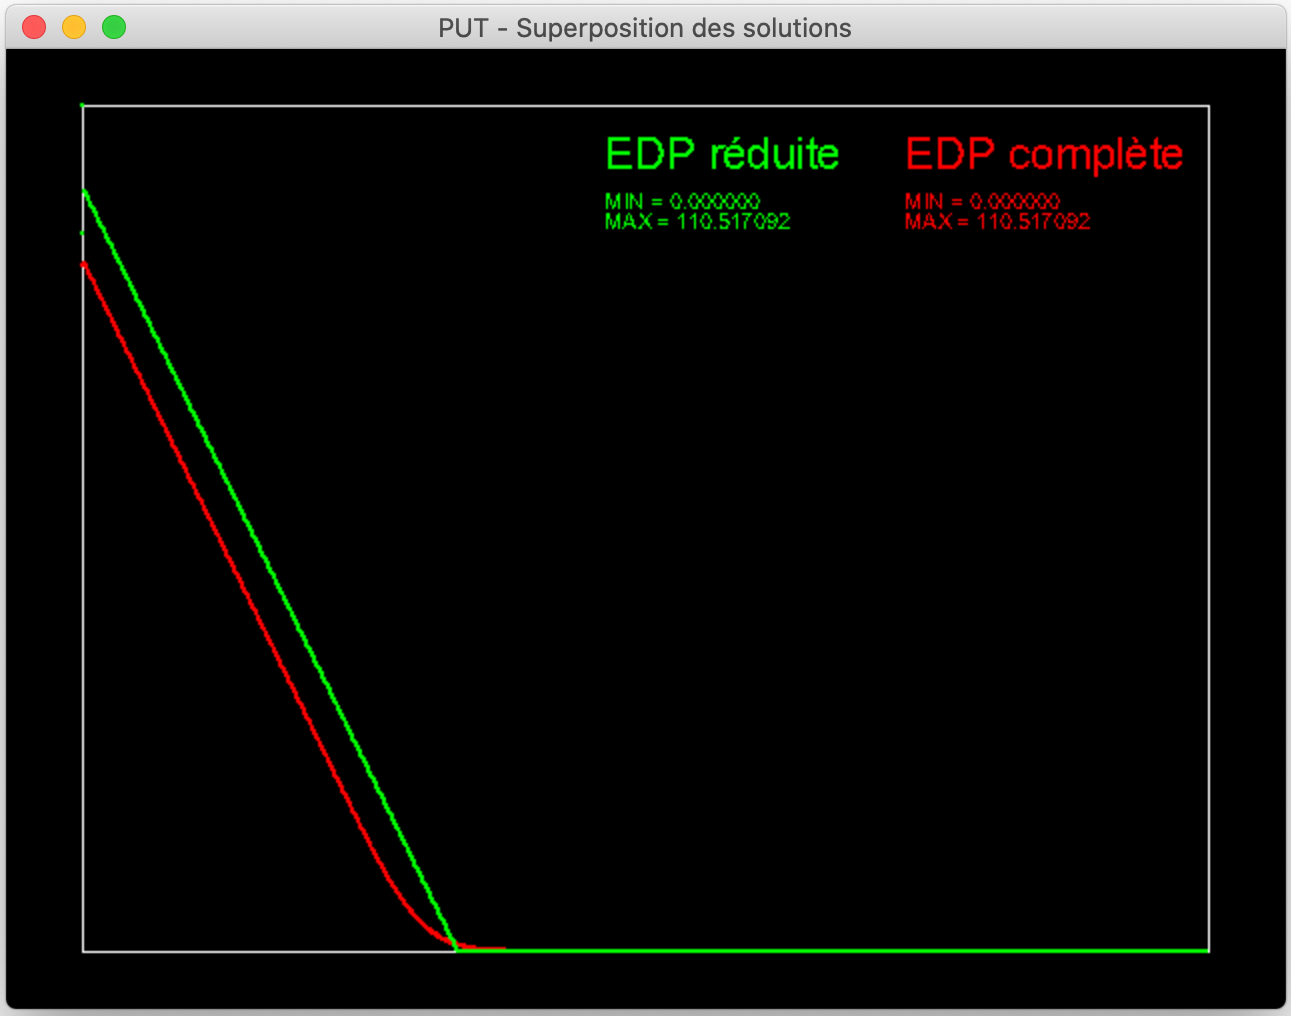
\includegraphics[scale = 0.27]{img/put_solutions.png}
    \caption{Courbes des 2 solutions pour un Put européen}
\end{figure}

\begin{figure}[h]
    \centering
    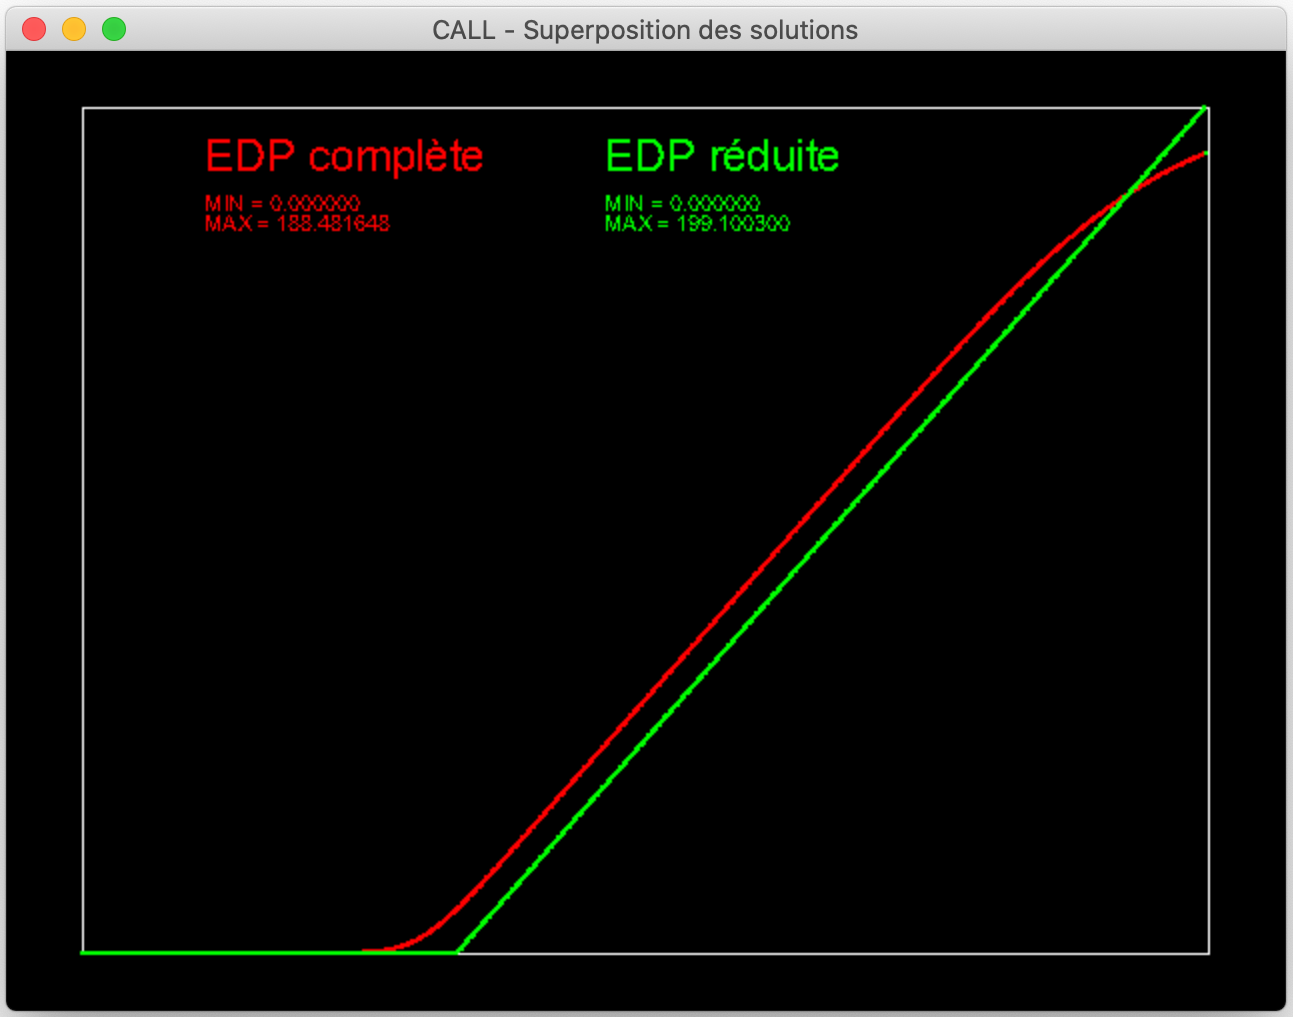
\includegraphics[scale = 0.27]{img/call_solutions.png}
    \caption{Courbes des 2 solutions pour un Call européen}
\end{figure}


\newpage


\section{Conclusion}
\subsection{Commentaires sur les résultats}
Au travers des 2 graphiques présentés en Annexes, on observe que l'erreur relative entre les 2 méthodes ne dépasse pas 10 unités dans chacun des cas.
On peut donc conclure que les 2 pricers présentent des résultats relativement similaires. De plus, les résultats trouvés sont très représentatifs de ceux présents dans la littérature en mathématiques financières.

En exportant les données trouvées sur des fichiers CSV puis en les exploitant avec un petit script en Python, nous trouvons que l'erreur moyenne est de $2.4$ sur chacune des situations, ce qui nous confortent dans notre conclusion.

\subsection{Commentaires personnels \& Synthèse générale des travaux}
Ce projet nous a permis de réaliser une vaste étude bibliographique puis d'étudier, de concevoir la structure, d'implémenter la solution puis de présenter les résultats sous forme graphique, en l'espace de moins de trois semaines.


L'erreur relative entre les 2 courbes ne dépassant pas 10 dans chacun des cas, nous pouvons conclure qu'il s'agit d'un excellent résulat et que la superposition des 2 courbes solutions, bien qu'imparfaite, témoigne d'une bonne implémentation. En restituant les solutions trouvées dans le contexte de l'étude réalisée, on s'aperçoit qu'il s'agit d'un prix; or, un écart de prix trouvés de 10 euros semble difficilement tolérable dans des systèmes de pricing d'options, qui obéissent à des contraintes de justesse et de conformité extrêmement fortes.

Afin de corriger ces erreurs, il faudra sans aucun doute considérer l'étude d'un $\theta$-schéma avec $\theta \neq \frac{1}{2}$, en trouvant une valeur optimale du paramètre de la méthode.

\section{Annexes techniques}

\begin{figure}[h]
    \centering
    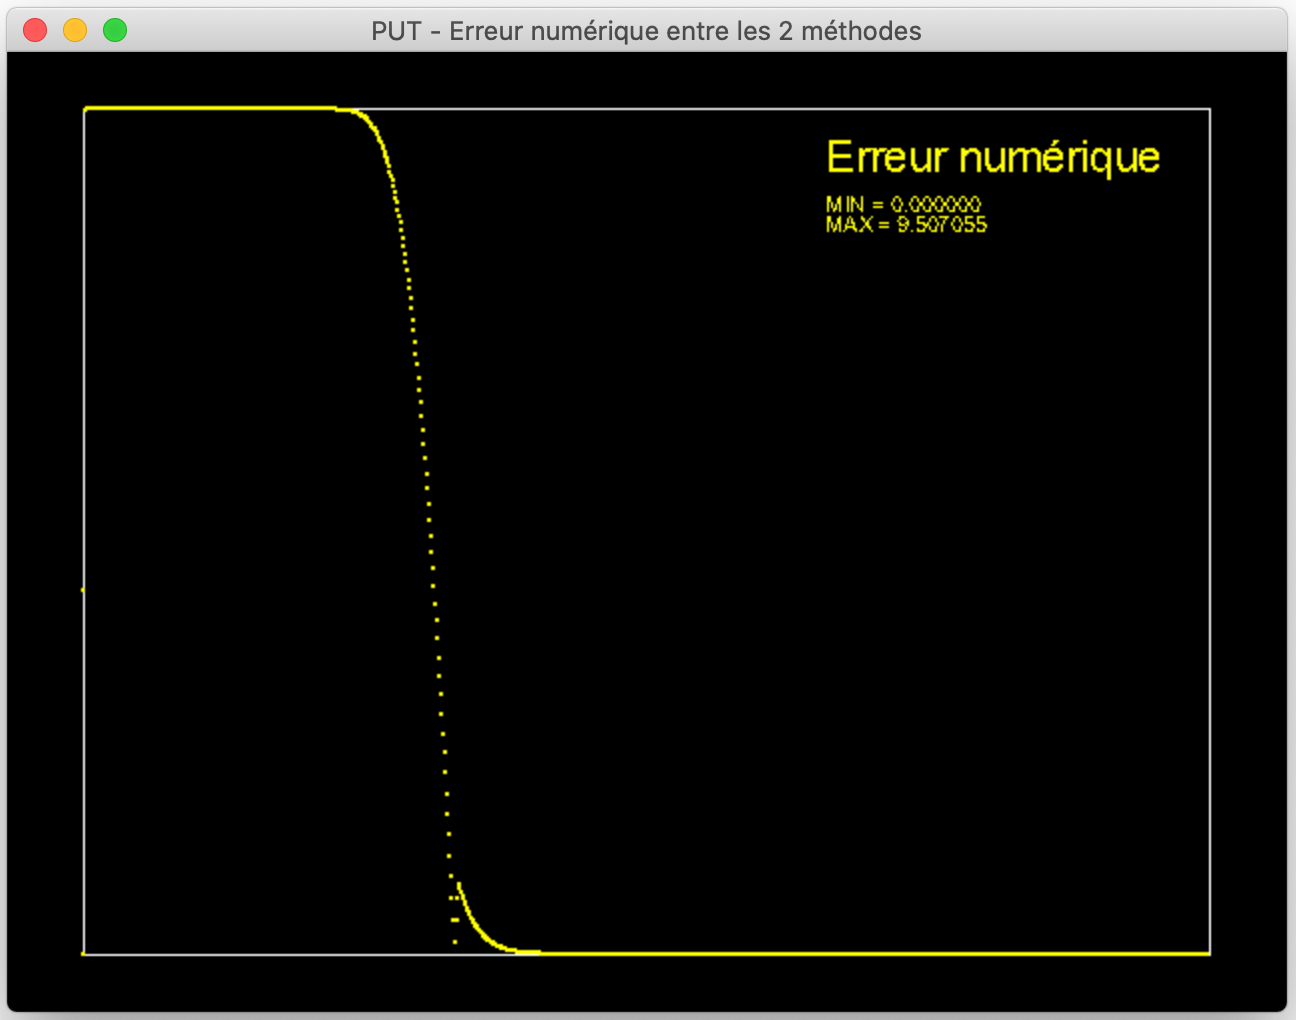
\includegraphics[scale = 0.27]{img/put_error.png}
    \caption{Erreur absolue entre les 2 solutions trouvées pour un Put européen}
\end{figure}

\begin{figure}[h]
    \centering
    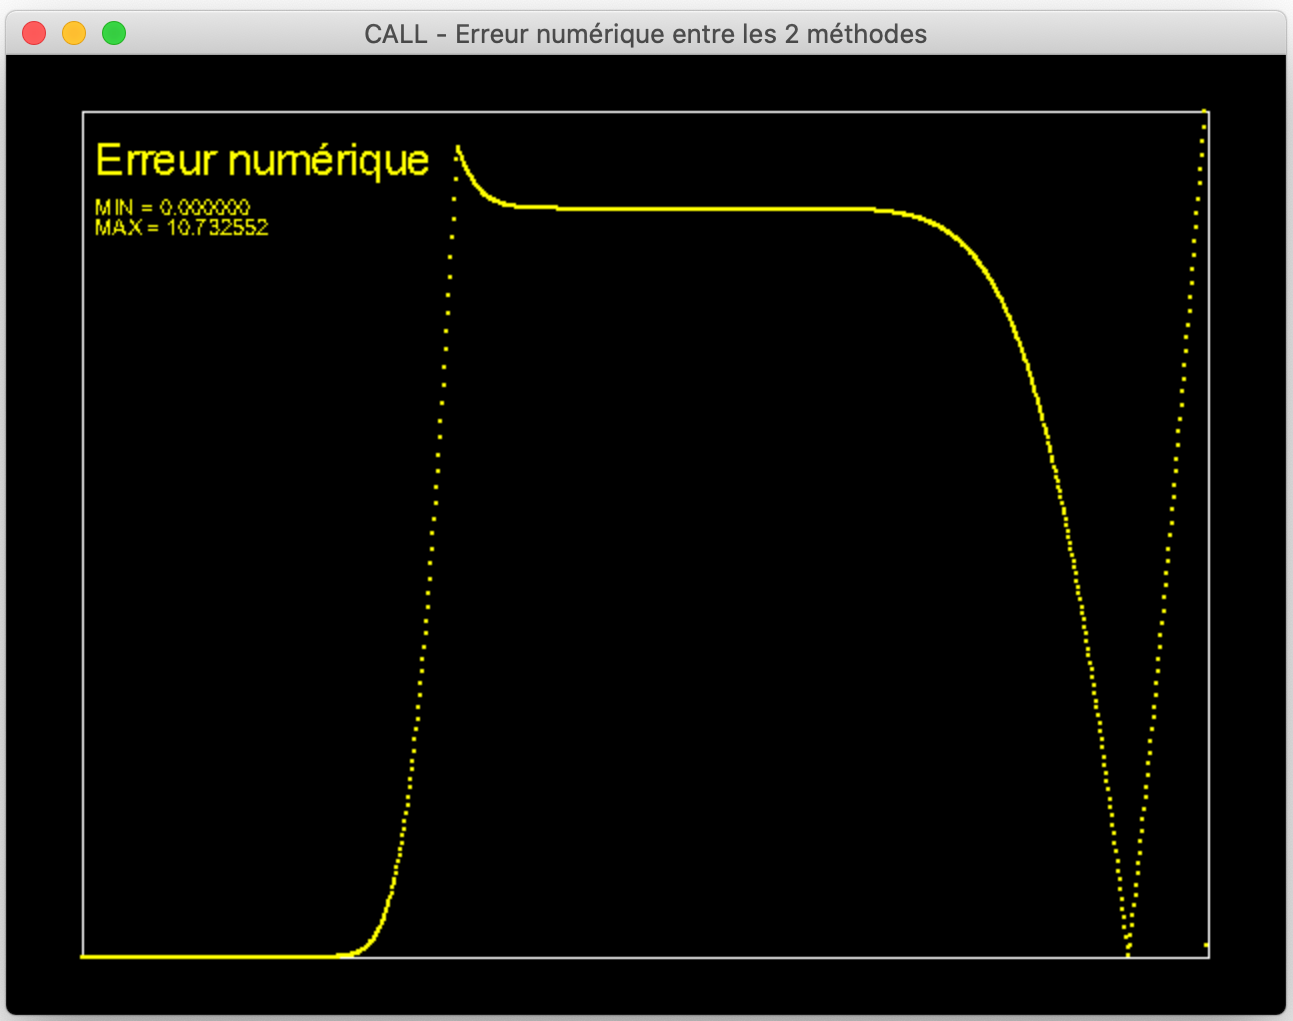
\includegraphics[scale = 0.27]{img/call_error.png}
    \caption{Erreur absolue entre les 2 solutions trouvées pour un Call européen}
\end{figure}


Le diagramme de classes UML est disponible ci-dessous.
\begin{rmq}
Les classes abstraites figurent en couleur orange.
\end{rmq}
\begin{landscape}
\begin{figure}
    \centering
    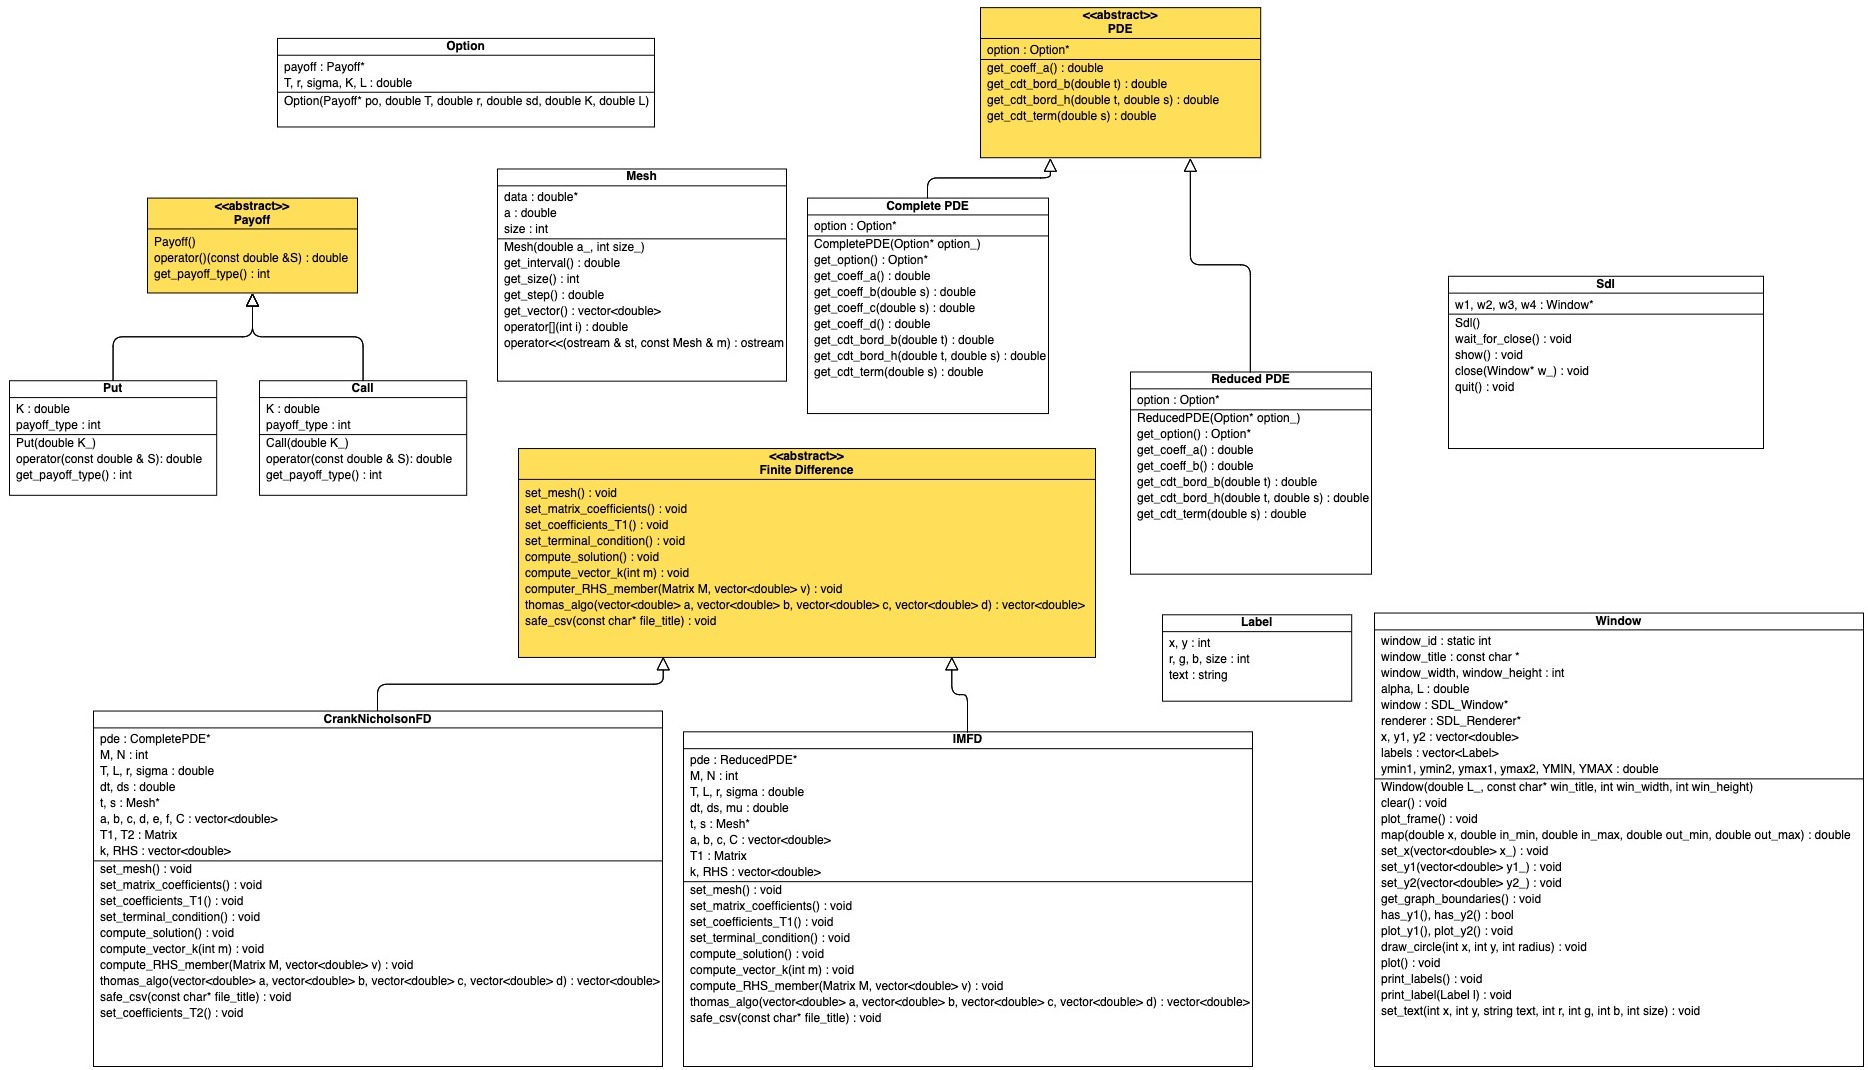
\includegraphics[scale = 0.4]{img/uml_diagram.jpg}
\end{figure}
\end{landscape}
\end{document}
